%************************************************
\chapter{Pulsar timing arrays} \label{chp:PTAs}
%************************************************

\begin{flushright}
	\slshape
	Wissen ist Nacht!\\ \medskip
	--- Leitspruch der Dunkelheitsforschung,\\
	Prof.~Dr.~Abdul Nachtigaller
\end{flushright}


In June 2023, a significant milestone was achieved in the field of \ac{GW} science and astrophysics: at an internationally acclaimed press conference the first evidence for the \graffito{The nHz signal} detection of a stochastic \ac{GW} background in the nano-Hertz frequency band was unveiled. On the same day, multiple collaborations, including the North American \acs{NANOGrav}~\cite{NANOGrav:2023gor}, the Australian \acs{PPTA}~\cite{Reardon:2023gzh}, the European \acs{EPTA} in conjunction with the Indian \acs{InPTA}~\cite{EPTA:2023fyk}, and the Chinese \acs{CPTA} collaboration~\cite{Xu:2023wog}, released their latest data sets, all of which support this groundbreaking discovery.

In the first section of this chapter (section~\ref{sec:PTAhistory}), we provide a brief overview of the history and current status of \acp{PTA}. Following that, in section~\ref{sec:singleGWPTA}, we explain how a monochromatic plane \ac{GW} can manifest itself in the timing data of a single observed pulsar. In section~\ref{sec:GWBPTA}, we express a stochastic \ac{GW} signal as a superposition of plane waves, \graffito{Contents of this chapter} leading to the characteristic \ac{HD} correlation function, for which \acp{PTA} have recently announced to have found evidence. Section~\ref{sec:PTAlikelihood} discusses the statistical methods used to separate a \ac{GWB} from other noise sources in a \ac{PTA}. A review of the latest results from the \ac{NANOGrav} collaboration is presented in section~\ref{sec:evidenceGWB}. Finally, in section~\ref{sec:SMBHBs}, this chapter concludes with a brief summary of the novel signal’s interpretation as an astrophysical background of \acp{SMBHB}, being the strongest contender for alternative cosmological interpretations.

\section{A short history of pulsar timing} \label{sec:PTAhistory}

In 1967 Jocelyn Bell, then a PhD student under Antony Hewish, made a groundbreaking discovery by identifying the first pulsar J1921+2153~\cite{Hewish:1968bj}. She observed radio sources with a very regular period of $1.337 \, \text{s}$. At the time, such regular fluctuations in radio signals were often \graffito{The first pulsar} attributed to human activity rather than astronomical sources. Within the following years of her discovery, more pulsars were identified thanks to rapid advancements in radio astronomy. In particular, also the aforementioned Hulse-Taylor binary pulsar J1915+1606 which led to the first indirect discovery of \acp{GW}~\cite{Hulse:1974eb}, rewarded with a Nobel Prize in 1993, was observed only a few years after Bell's initial discovery.

Already in the early 1930s, three decades before Bell's discovery, the existence of neutron stars had been hypothesized by Landau, Baade, and Zwicky~\cite{Landau:1932uwv, Baade:1934}. Just a few months before Bell's discovery, Pacini and Gold proposed the existence of rapidly rotating neutron stars which would emit pulses of electromagnetic radiation~\cite{Pacini:1968, Gold:1968zf}. The origin \graffito{Pulsars are spinning neutron stars} of their fast rotations is now understood to be due to the conservation of angular momentum from their progenitor stars, which become more compact and faster-spinning as the nuclear fusion within them ceases~\cite{Lorimer:2004}.

Neutron stars are sources of strong dipolar magnetic fields of up to $10^{11} \, \text{T}$, whose axis is not necessarily aligned with the star's axis of rotation. The neutron star can thus be modeled as a precessing magnetic dipole, which in turn generates an electric field. \graffito{The lighthouse model} The latter accelerates charged particles within the neutron star's magnetosphere, exciting beams of electromagnetic radiation in the radio band along the magnetic dipole's direction, effectively turning the neutron star into a lighthouse sweeping radio beams through its host galaxy~\cite{Goldreich:1969sb}.

Typical pulsars have an orbital period of $P \simeq 0.1 - 1 \, \text{s}$ and a spin-down rate of $\dot{P} \simeq 10^{-15}$, meaning their periods increase only by about $1 \, \text{ns}$ per month due to their \graffito{Millisecond pulsars} high moment of inertia. Additionally, there is a population of millisecond pulsars which rotate much faster ($P \simeq 10 \, \text{ms}$), resulting in an even more stable orbital period ($\dot{P} \simeq 10^{-20}$). These millisecond pulsars are typically formed in binary systems where a regular pulsar accretes mass from its companion, thus gaining angular momentum from the binary system~\cite{Lorimer:2004}. 

Due to the stability of their orbital periods, the sequence of pulses from millisecond pulsars can be predicted with extreme precision using a timing model. These models account for factors like spin-down $\dot{P}$ and higher time-derivatives of the period $P$, the effects of the ionized interstellar medium, Earth's proper motion, and possible delays from the orbital motion of binary pulsars. Importantly, \acp{GW} also affect the arrival times of these pulses, a phenomenon known since the late 1970s~\cite{Sazhin:1978myk, Detweiler:1979wn}. The \graffito{Hellings and Downs} work of Hellings and Downs in the early 1980s provided a method to distinguish the effect of a \ac{GW} background on arrival times from other noise sources~\cite{Hellings:1983fr}: By correlating timing residuals between several pulsars, a characteristic pattern due to the quadrupolar nature of gravitational radiation was predicted to be observable in case a \ac{GWB} alters the time intervals between pulses.

This led to the concept of \acp{PTA} in the late 1980s~\cite{Foster:1990}, which promised to be able to disentangle the effects of clock errors (monopolar correlation)~\cite{Hobbs:2019ktp}, a mismodeling of the Solar System's barycenter (dipolar correlation)~\cite{Caballero:2018lvc}, and the searched-for \ac{HD} correlation of \acp{GW}. \graffito{The \ac{PTA} idea} Today, several \ac{PTA} collaborations exist, namely \acs{NANOGrav}, \acs{PPTA}, \acs{EPTA}, \acs{InPTA}, and \acs{CPTA}. Each collaboration observes a set of pulsars using radio telescopes, sometimes in various radio frequency bands. These collaborations (except for \acs{CPTA} which acts as an observer) share their data under the \ac{IPTA} framework, thus drastically increasing the number of possible pulsar cross-correlations.

The lowest \ac{GW} frequency a \ac{PTA} can detect is determined by the inverse time span of the arrival data, $f \gtrsim 1 / T$. For an indicative observational period of $T = 10 \, \text{yr}$, the lowest detectable frequency is slightly below $3 \, \text{nHz}$. Lower-frequency \acp{GW} cannot be detected through pulsar timing variations but rather manifest themselves as contributions to the pulsar spin-down rate $\dot{P}$ and higher derivatives \graffito{nHz to µHz} of the period $P$. Thus, \acp{PTA} are generally not sensitive to lower-frequency \acp{GW}. The upper frequency limit is determined by how often a pulsar is observed, typically every few weeks or even once per week in the case of \acs{EPTA}. The highest observable \ac{GW} frequency is thus around $50 \,  \text{yr}^{-1} \simeq 1 \, \text{µHz}$. However, sensitivity is lower at these frequencies due to noise-dominated timing residuals, i.e.~the difference between the timing model and the actually observed \acp{TOA} of pulses.

In their latest data release, the \ac{NANOGrav} collaboration found evidence for a \ac{GW} background with an amplitude of around $h^2 \Omega_\gw \simeq 10^{-10} - 10^{-8}$ (see the previous fig.~\ref{fig:observability}). It is not yet clear whether the signal is of astrophysical or \graffito{An unexpectedly strong nHz background} cosmological origin. The prevailing null hypothesis for the signal's origin is an astrophysical background of \acsp{SMBHB}~\cite{NANOGrav:2023pdq}. However, due to the unexpectedly high amplitude and low spectral index of the measured signal, as well as unresolved issues like the final parsec problem (see sec.~\ref{sec:finalpc}), this interpretation has been questioned~\cite{NANOGrav:2023hvm}.


\section{Gravitational wave effects on a single pulsar's timing} \label{sec:singleGWPTA}

We will now study the effect of \acp{GW} on a pulsar's emitted radio pulses. Before we study the effect of a stochastic background on a pulsar timing array, let us first consider the effect of a monochromatic and plane \ac{GW} on a single pulsar's period. We will identify the coordinate origin with the barycenter of the Solar System (often referred to as \textit{Earth} in the pulsar timing literature for simplicity) and refer to the pulsar position with $\bm{x} = \bm{n}_a$. The label $a$ will allow us to generalize and correlate between two pulsars in the following \graffito{We work in \ac{TT} gauge} section. We further work in \ac{TT} gauge, such that the coordinate distances $d_a$ between Earth and pulsars remain constant, whereas the proper distance between them oscillates. In that sense the following calculation is very similar to the one performed in section~\ref{sec:GWinvac} and analogous to studying the response of a single interferometer arm to a \ac{GW}. Both this and the following subsection are close to the calculations presented in~\cite{Maggiore:2018sht, Taylor:2021yjx}.

For a radio pulse moving in $x$-direction, the line element reads \graffito{A pulse moving along the $x$-axis}
\begin{align}
	0 = - \diff t^2 +\ba{ \delta_{ij} + h_{ij}^\TT} \diff x^i \diff x^j = - \diff t^2 +\ba{ 1 + h_{xx}^\TT} \diff x^2 \, .
\end{align}
The pulse moves from $\bm{x}$ to the coordinate origin, so ignoring the effect of the metric perturbation we can write $\bm{x}(t) \simeq (t_\text{obs} - t) \hat{\bm{x}}$. To first order in the metric perturbation we obtain
\begin{align}
	\diff x = - \sqrt{\frac{\diff t^2}{1 + h_{xx}^\TT(t, \bm{x}(t))}} = \ba{1 - \frac{h_{xx}^\TT(t,\bm{x}(t))}{2}} \diff t \, .
\end{align}
By integrating this expression from the emission of the radio pulse at $t_\text{em}$ to the time of observation $t_\text{obs} \simeq t_\text{em} + d_a$, ignoring the effect of the metric perturbation in the integral boundary, we can obtain $t_\text{obs}$ to first order in the metric perturbation,
\begin{align}
	t_\text{obs} = t_\text{em} + d_a + \frac{1}{2} \int_{t_{\text{em}}}^{t_{\text{obs}}} \diff t^\prime h_{xx}^\TT(t^\prime,\bm{x}(t^\prime)) \, . 
\end{align}
We can easily generalize this expression to \graffito{A pulse moving in direction $\hat{\bm{n}}_a$} the case of a radio pulse in direction $\hat{\bm{n}}_a$ not necessarily coinciding with the $x$-axis by replacing $h_{xx}^\TT \rightarrow n_a^i n_a^j h_{ij}^\TT$, yielding 
\begin{align}
	t_\text{obs} = t_\text{em} + d_a + \frac{n_a^i n_a^j}{2} \int_{t_{\text{em}}}^{t_{\text{obs}}} \diff t^\prime h_{ij}^\TT(t^\prime,\ba{t_\text{em} + d_a - t^\prime} \hat{\bm{n}}_a) \, . 
\end{align}
The difference between $t_\text{obs}$ and the observation time $t_\text{obs}^\prime$ of another \graffito{The delay $\Delta P_a$ of a single pulse} radio pulse emitted at $t_\text{em}^\prime = t_\text{em} + P_a$ hence reads $t_\text{obs}^\prime - t_\text{obs} = P_a + \Delta P_a$ with 
\begin{align}
	\Delta P_a = \frac{n_a^i n_a^j}{2} \int_{t_{\text{em}}}^{t_{\text{obs}}} \diff t^\prime \bb{ h_{ij}^\TT(t^\prime + P_a, \bm{x}_a(t^\prime)) -h_{ij}^\TT(t^\prime, \bm{x}_a(t^\prime))}  \, ,
\end{align}
where $\bm{x}_a(t^\prime) = \ba{t_\text{em} + d_a - t^\prime} \hat{\bm{n}}_a$. Since the \ac{GW} frequency is $f\simeq \mathcal{O}(\text{nHz})$, while the pulsar's rotational period is at the scale of $P_a \simeq \mathcal{O}(\text{ms})$, their product $f P_a \simeq 10^{-9}$ is tiny. Therefore, it is enough to expand the metric perturbation around $t^\prime$ to first order in $f P_a$ to find an expression for the relative delay
\begin{align}
	\frac{\Delta P_a}{P_a} = \frac{n_a^i n_a^j}{2} \int_{t_{\text{em}}}^{t_{\text{obs}}} \diff t^\prime\bb{ \pd{}{t^\prime} h_{ij}^\TT(t^\prime, \bm{x})}_{\bm{x} = \bm{x}_a(t^\prime)} 
\end{align}
between two pulses. A \ac{GW} $h_{ij}^\TT(t, \bm{x}_a) = \mathcal{A}_{ij}(\hat{\bm{n}}) \, \cos \ba{2 \pi f \ba{t - \hat{\bm{n}} \bm{x}_a}}$ propagating in $\hat{\bm{n}}$-direction hence induces a (sometimes referred to as \textit{red}-) shift $z_a \equiv \frac{\Delta P_a}{P_a}$ of the pulse's \ac{TOA} reading
\begin{align}
	 z_a &= \frac{n_a^i n_a^j \mathcal{A}_{ij}(\hat{\bm{n}})}{2 \ba{1 + \hat{\bm{n}} \cdot \hat{\bm{n}}_a }} \bb{\cos \ba{2 \pi f t_\text{obs}} - {\cos \ba{2 \pi f t_\text{em} - 2 \pi f \tau_a \hat{\bm{n}}_a \cdot \hat{\bm{n}}}}} \\
		&=  \frac{n_a^i n_a^j}{2 \ba{1 + \hat{\bm{n}} \cdot \hat{\bm{n}}_a }} \bb{h_{ij}^\TT(t_\text{obs}, \bm{x} = 0) - h_{ij}^\TT(t_\text{obs} - \tau_a, \bm{x}_a)} \label{eq:PTAredshift}
\end{align}
with $\tau_a = t_\text{obs} - t_\text{em} \sim \text{kpc} \sim 10^3 \, \text{yr}$ being the runtime of the radio signal. The first term is usually referred to as the Earth term, as it only depends on the local metric perturbation at the time of observation. In practice, the coordinate origin is however set to the barycenter of the Solar System, from which the time delay $z_a$ at Earth can be inferred by translating into a rotating reference frame in the deterministic timing model discussed in section~\ref{sec:PTAlikelihood}. This is done by adding up the effects of a Rømer time delay due to the annual motion of the \graffito{The ``Earth'' term and the pulsar term} Earth around the Sun, a Shapiro time delay due to the Solar System's own gravitational field, and an Einstein time delay due to the detectors proper motion around the Sun and the difference between coordinate time and proper time on Earth~\cite{Taylor:2021yjx}. The second term in eq.~\eqref{eq:PTAredshift}, referred to as the pulsar term, depends on the metric perturbation at the location of the pulsar at the time of the pulse's emission, several thousand years ago.

\section{Effect of a GWB on an array of pulsars} \label{sec:GWBPTA}
We can now apply eq.~\eqref{eq:PTAredshift} to the case of a stochastic \graffito{Expanding in plane waves} \ac{GWB}. Using the plane wave expansion~\eqref{eq:planewaveexpansion} and replacing $t_\text{obs}$ for $t$, we immediately obtain 
\begin{align}
	z_a(t) &= \sum_{A= +, \times} \int_{-\infty}^{\infty} \diff f \int \diff^2 \hat{\bm{n}} \, \tilde{h}_A(f, \hat{\bm{n}}) \,  F_a^A(\hat{\bm{n}}) \,  \mathrm{e}^{-2 \pi \mathrm{i} f t}  \nonumber \\ & \quad \times \ba{1 - \mathrm{e}^{2 \pi \mathrm{i} f \tau_a \ba{1 + \hat{\bm{n}} \cdot \hat{\bm{n}}_a}}} \label{eq:za}
\end{align}
with the antenna response pattern function for pulsar $a$
\begin{align}
	 F_a^A(\hat{\bm{n}}) \equiv \frac{n_a^i n_a^j e_{ij}^A(\hat{\bm{n}})}{2 \ba{1 + \hat{\bm{n}} \cdot \hat{\bm{n}}_a}}  \, . \label{eq:ARPf}
\end{align}
As discussed previously, a Gaussian stochastic \ac{GWB} is only characterized through its variance and mean, the latter of which we deliberately set to zero. Hence we need to compute the correlator $\ev{z_a(t) z_b(t)}$ to make progress, where the brackets refer to an ensemble average over realizations of the stochastic variable $\tilde{h}_A(f, \hat{\bm{n}})$. Plugging \graffito{A \ac{GW} background is characterized by its variance} in the previous parameterization of the variance of a stationary, isotropic and unpolarized \ac{GW} background from eq.~\eqref{eq:ensembleaverage}, we obtain the correlator
\begin{align}
	\ev{z_a(t) z_b(t)} = \int_{0}^{\infty} \diff f \, S_{h}(f) \int \frac{\diff^{2} \hat{\bm{n}}}{4 \pi} \, \mathcal{K}_{a b}(f ; \hat{\bm{n}}) \sum_{A=+, \times} F_{a}^{A}(\hat{\bm{n}}) F_{b}^{A}(\hat{\bm{n}})\\
	\text{with} \qquad 
	\mathcal{K}_{a b}(f ; \hat{\bm{n}})=\bb{1-\mathrm{e}^{-2 \pi \mathrm{i} f \tau_{a} \ba{1+\hat{\mathbf{n}} \cdot \hat{\mathbf{n}}_{a}}}} \bb{1-\mathrm{e}^{2 \pi \mathrm{i} f \tau_{b} \ba{1+\hat{\mathbf{n}} \cdot \hat{\mathbf{n}}_{b}}}} \, .
\end{align}
The function $\mathcal{K}_{ab}$ is quickly oscillating with $f \tau_a \gtrsim 10$ for $f \gtrsim 1 \, \text{nHz}$ and $\tau_a > 0.1 \, \text{kpc}$ even for the closest observed pulsar. Unless $\abs{1 + \hat{\mathbf{n}} \cdot \hat{\mathbf{n}}_{a} } \lesssim 1/10$, i.e.~unless the \ac{GW} comes straight from the direction of the pulsar under consideration, we obtain $\mathcal{K}_{ab} \rightarrow 1$ for $a \neq b$. For $a = b$, one instead obtains the auto-correlation limit $\mathcal{K}_{ab} \rightarrow 2$.  \graffito{$\mathcal{K}_{ab} \rightarrow 1 + \delta_{ab}$}  Since $f \tau_a$ is large for most pulsars under consideration, we can hence safely set  $\mathcal{K}_{ab}(f; \hat{\bm{n}}) \rightarrow 1 + \delta_{ab}$ and concentrate on the remaining integral over the product of detector pattern functions $F_{a}^{A}(\hat{\bm{n}}) F_{b}^{A}(\hat{\bm{n}})$. This integral is elementary, but still requires a tedious calculation at whose end one arrives at the overlap reduction formula
\begin{align}
	 \Gamma_{ab} &\equiv \frac{3}{2} \int \frac{\diff^{2} \hat{\bm{n}}}{4 \pi} \, \mathcal{K}_{a b}(f ; \hat{\bm{n}})  \sum_{A=+, \times} F_{a}^{A}(\hat{\bm{n}}) F_{b}^{A}(\hat{\bm{n}}) \\
	 &=\frac{3}{2} x_{ab} \ln x_{ab} - \frac{1}{4} x_{ab}  + \frac{1}{2} \delta_{ab} + \frac{1}{2} \label{eq:HD}
\end{align}
with $x_{ab} = \frac{1}{2} \ba{1 - \cos \theta_{a b}}$, where $\theta_{a b}$ is the angle between pulsars $a$ and $b$ as seen from Earth. The function $\Gamma(x_{ab})$ was first \graffito{The \ac{HD} curve} derived by Hellings and Downs~\cite{Hellings:1983fr} (for $a \neq b$) and is since known as the \ac{HD} curve. The prefactor $\frac{3}{2}$ was introduced to ensure the normalization to $\Gamma_{ab} = 1$ for $a = b$.

In fig.~\ref{fig:hd} the \ac{HD} curve is plotted in comparison to a monopolar and a dipolar correlation function. A flat monopolar correlation would show up in the data analysis of a \ac{PTA} in the case of clock errors which affect all pulse timestamps in the same way, corresponding to a maximal correlation between pulsars regardless of the specific pulsar pair. A dipolar correlation would instead indicate a mismodeling of the barycenter of the Solar System, leading to a secular motion of Earth with respect to the pulsars. Note that the \ac{HD} curve is not a pure quadrupolar correlation function, \graffito{Interpreting the \ac{HD} curve} as can be seen by it reaching 0.25 instead of 0.5 for two pulsars in opposite directions. Using a decomposition into Legendre polynomials one can however show that the \ac{HD} curve can be well approximated as the sum of a quadrupolar and an octupolar term~\cite{Taylor:2021yjx}. The reason for the occurrence of the octupole and higher-order multipolar correlations is that the denominator in the antenna response pattern~\eqref{eq:ARPf} implies that there is a preferred direction $\hat{\bm{n}} \cdot \hat{\bm{n}}_a = -1$, in which the response of the detector system of Earth and pulsar is largest. Note also that the maximum of the \ac{HD} curve is reached only in the case of an auto-correlation $a = b$. Even pulsar  pairs with a low angular separation can have a maximum cross-correlation of 0.5, because the product of two pulsar terms in $\mathcal{K}_{ab}$ decorrelates quickly for pulsars with a separation larger than a \ac{GW} wavelength~\cite{Mingarelli:2014xfa}.

\begin{figure}[t]
	\centering
	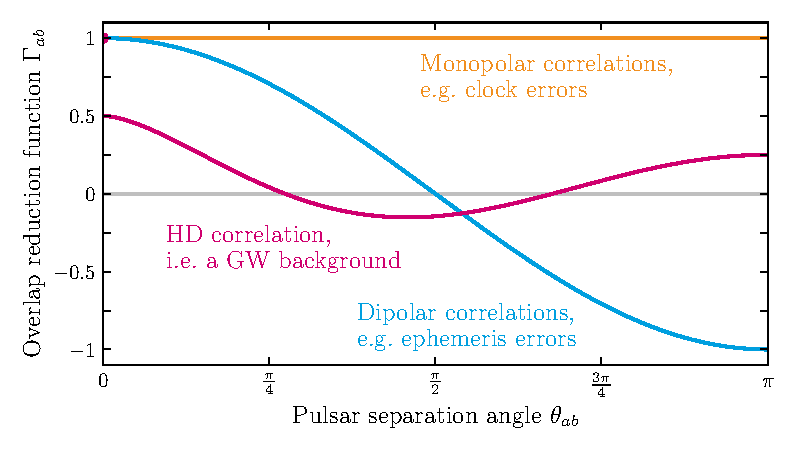
\includegraphics[width=\textwidth]{thesisplots/HD/HD}
	\caption{Comparison of the \ac{HD} curve from eq.~\eqref{eq:HD}, a monopolar, and a dipolar correlation function. The latter two would for instance be expected if clock errors or Solar System ephemeris errors affected the \acp{TOA} instead of a \ac{GW} background.}
	\label{fig:hd}
\end{figure}

For the correlator of shifts of pulse arrival rates we hence obtain
\begin{align}
	\ev{z_a(t) z_b(t)} = \frac{2}{3} \Gamma_{ab} \int_0^\infty \diff f \, S_h(f) \, .
\end{align}
However, a \ac{PTA} \graffito{The timing residual $R_a$ and its variance $r_{ab}$} is not able to directly measure the shift $z_a$ of a single pulse. Instead, it measures pulse arrival times, which shift from their regular pattern due to the  accumulated timing residual
\begin{align}
	R_a(t) \equiv \int_0^t \diff t^\prime z_a(t^\prime) \label{eq:tresidual} \, .
\end{align}
The quantity of interest to connect the previous considerations with actual \ac{PTA} measurements is hence $r_{ab}(t) = \ev{R_a(t) R_b(t)}$. Plugging in the definition of $R_a(t)$ and eq.~\eqref{eq:za} for $z_a(t)$ we obtain the variance
\begin{align}
	r_{ab}(t) =  \frac{2}{3} \Gamma_{ab} \int_0^\infty \diff f \,\frac{ S_h(f)}{\ba{2 \pi f}^2} 2 (1 - \cos (2 \pi f t)) \, .
\end{align}
The time dependence occurs here due to the arbitrary lower integration boundary in the above definition of $R_a(t)$. Considering that the \ac{PTA} only is sensitive to \acp{GW} in a frequency band in which $2 (1 - \cos (2 \pi f t)) = \mathcal{O}(1)$, one obtains~\cite{Maggiore:2018sht}
\begin{align}
	r_{ab} \simeq \int_{0}^{\infty} \diff f \, S_{ab}(f) \quad \text{with} \quad S_{ab}(f) \equiv \frac{2}{3} \Gamma_{ab}  \frac{S_h(f)}{(2 \pi f)^2} \, .
\end{align}
The function $S_{ab}(f)$ is referred to as the \graffito{The timing-residual cross-power spectral density $S_{ab}(f)$} timing-residual cross-power spectral density and has units of $\text{s}^3$. \ac{PTA} collaborations often work with the parameterization $\Phi_{ab}(f) = S_{ab}(f)/T$ (with units of $\text{s}^2$) when doing their data analysis, where $T = \mathcal{O}(10 \, \text{yr})$ is the total data set time span. The effect of the overlap reduction function can easily be factored out of this expression, $\Phi_{ab}(f) = \Gamma_{ab} \Phi(f)$,  due to the previously identified approximate frequency-independence of $\mathcal{K}_{ab}$. The remaining spectrum $\Phi(f)$ (not carrying pulsar indices) only captures the effect of a given \ac{GW} mode with frequency $f$ on the variance on the timing residuals. The quantity $\rho(f) = \sqrt{\Phi(f)}$ in units of time is often referred to as the excess timing delay.

Expressing the \ac{GW} spectrum  through its characteristic strain amplitude $h_\text{c}(f)$ or its energy density spectrum $h^2 \Omega_\gw(f)$, see eq.~\eqref{eq:specconversion}, we end up with the following expressions for the excess timing delay
\begin{align}
	\rho(f) = \sqrt{\frac{S_h(f)}{6 \pi^2 f^2 T}} = \sqrt{\frac{h_\text{c}^2(f)}{12 \pi^2 f^3 T}} = \sqrt{\frac{H_{100}^2}{8 \pi^4 f^5 T} \,  h^2 \Omega_\gw(f)} \, .  \label{eq:rhof}
\end{align}
Given a \graffito{The excess timing delay $\rho(f)$ and its relation to $\Omega_\mathrm{gw}(f)$} measurement of $\rho(f)$, we can hence easily infer the underlying \ac{GW} spectrum. Typical values of $\rho(f)$ that \acp{PTA} quote are between $1 \, \text{ns}$ and $1 \, \text{µs}$ for frequencies in the range $1 - 30 \, \text{nHz}$ (see for instance fig.~\ref{fig:spectrum_correlations_plot} in the following section).

Note that in the above calculation we assumed that the stochastic \ac{GWB} under consideration is isotropic. In case the \ac{GWB} is instead of astrophysical origin, this assumption cannot be sustained and a more generalized overlap reduction formula needs to be used. In the presence of anisotropies, \graffito{Generalizing the overlap reduction formula} one finds that the overlap reduction formula becomes a function of the individual pulsars' positions on the celestial sphere~\cite{Bernardo:2022xzl}. Further, \ac{GR} modifications which lead to \acp{GW} with more than two propagating tensorial metric components lead to a dependence of the overlap reduction formula on the pulsar distances and the \ac{GW} frequency, rendering searches for the \ac{HD} correlation and deviations from it a powerful probe of new physics in their own right~\cite{Bernardo:2023mxc}. Within this thesis, we will only consider the \ac{HD} curve as a possible overlap reduction formula or set $\Gamma_{ab} = \delta_{ab}$ for computational reasons to be explained in the next section, thus ignoring the effect of the \ac{GW} polarization on the pulse arrival times, when trying to fit them to a specific backgrounds $h^2 \Omega_\gw(f)$ in chapters \ref{chp:ptabbn} and \ref{chp:pbh}.

\section{The PTA likelihood} \label{sec:PTAlikelihood}


In the above derivation we assumed that only \acp{GW} \graffito{Separating deterministic signals from interesting noise} lead to a change of the arrival times of a given pulsar's radio pulses. This is obviously an oversimplification. In  practice, the mechanisms which predict the \ac{TOA} of a pulse are a combination of both deterministic \textit{and} stochastic processes, the latter of which include the effect of \acp{GW},\footnote{We will ignore the effect of continuous \acp{GW} (e.g. from a single close-by \ac{SMBHB} inspiral) for brevity, which would show up as an unmodeled contribution to the deterministic timing model. So far, no significant evidence for such continuous \acp{GW} has been found with \acp{PTA}~\cite{NANOGrav:2023pdq}.} 
\begin{align}
	t_{ai}^{\text{TOA}} = t_{ai}^{\text{det}} + \delta t_{ai}^{\text{stoch}} \, . \label{eq:detstoch}
\end{align}
The index $i$ here indicates the $i$-th pulse of pulsar $a$ with respect to an arbitrary initial point in time at which data taking starts. The goal of this section will now be to identify how a \ac{GW}-induced timing residual $R_a(t_i)$ (defined in eq.~\eqref{eq:tresidual}) contributes to the stochastic part $\delta t_{ai}^{\text{stoch}}$ of the \ac{TOA}. Eventually we will present how one can infer a \ac{GW} spectrum $h^2 \Omega_\gw(f)$ from pulsar timing data. To do so, we will summarize the analysis pipeline used by the \ac{NANOGrav} collaboration, described in detail in ref.~\cite{Taylor:2021yjx}. 

In a first step, a deterministic timing model needs to be found for each pulsar of the \ac{PTA}. To do so, there exist \graffito{Step 1: The timing model} the highly specialized codes \texttt{TEMPO}, \texttt{TEMPO2}~\cite{Hobbs:2006cd, Edwards:2006zg, Hobbs:2009yn} and \texttt{PINT}~\cite{Luo:2020ksx}. They allow to perform a fit of the observed \acp{TOA} $t_{ai}^{\text{TOA}}$ to a timing model (also referred to as timing ephemeris) $t_{ai}^{\text{det}}(\bm{\beta}_a)$, which depends on a set of deterministic timing parameters $\bm{\beta}_a$, including the period of the pulsar, its spindown, possible pulsar glitches, the aforementioned Solar System ephemeris, the precise position of the pulsar in the celestial sphere and its motion therein, as well as additional Keplerian parameters if the pulsar is part of a binary system. After performing a least-squares fit, one obtains the best-fit vector $\bm{\beta}_a^0$ and the corresponding timing residuals
\begin{align}
	\delta t_{ai} = t_{ai}^{\text{TOA}} - t_{ai}^{\text{det}}(\bm{\beta}_a^0) \label{eq:timingresidual}
\end{align}
for each pulsar.

No matter how accurate the first step is done, the process of finding a timing model is limited by it only including deterministic processes. \graffito{Step 2: Understanding the timing residuals} The found timing model will hence be very good, but not a perfect fit for the observed \acp{TOA} $t_{ai}^{\text{TOA}}$. Denoting the true (and unknown) timing ephemeris with $\bm{\beta}_a^\text{true}$ and interpreting the \ac{TOA} index $i$ as the component of a vector, we can write eq.~\eqref{eq:detstoch} as $\bm{t}_{a}^{\text{TOA}} = \bm{t}_{a}^{\text{det}}(\bm{\beta}_a^\text{true}) + \bm{\delta  t}_{a}^\text{stoch}$. Further, defining the difference between our initial timing model and the true model as $\bm{\epsilon}_a = \bm{\beta}_a^\text{true} - \bm{\beta}_a^0$ and plugging into eq.~\eqref{eq:timingresidual} we find
\begin{align}
	 \bm{\delta t}_{a} &= \bm{t}_a^\text{det} (\bm{\beta}_a^0 +   \bm{\epsilon}_a) - \bm{t}_a^\text{det} (\bm{\beta}_a^0) +\bm{\delta t}_{a}^\text{stoch} \nonumber \\
	&= M_a \bm{\epsilon}_a +\bm{\delta  t}_{a}^\text{stoch}  + \mathcal{O}(\bm{\epsilon}^2_a) \quad \text{with} \quad M_a = \left. \nabla_{\bm{\beta}_a} \bm{t}_a \right|_{\bm{\beta}_a^0} \, .
\end{align}
The design matrix $M_a$ has the shape ($N_\text{TOA} \times m$), where $N_\text{TOA}$ is the length of the vector $\bm{t}_{a}$ corresponding to the number of \acp{TOA} for pulsar $a$, and $m$ refers to the number of timing ephemeris parameters in $\bm{\beta}_a$.

The goal is now to identify \graffito{Stochastic noise sources are red or white} the different noise sources which contribute as random Gaussian processes in $\bm{\delta t}_{a}^\text{stoch}$, including a \ac{GWB}. Typically, one distinguishes between red and white noise sources,
\begin{align}
	\bm{\delta t}_{a}^\text{stoch} = \bm{\delta t}_{a}^\text{red} + \bm{\delta t}_{a}^\text{white} \, .
\end{align}
White noise is independent of the Fourier modes of $\bm{\delta t}_{a}^\text{stoch}$, whereas red noise instead has a frequency dependence and amplitude that is largest at the lowest frequencies. Red noise is therefore sourced by processes which operate on long timescales of the order of months to decades.

The white noise $\bm{\delta t}_{a}^\text{white}$ has \graffito{White noises} different sources connected to radiometer noise, instrumental effects, and pulsar phase jitter. Often, white noise sources are also referred to by their technical names \texttt{EFAC}, \texttt{EQUAD} and \texttt{ECORR}. The specific origins of these various noises are not central to the focus of this thesis. Let us only note here, that they are related to the specific combinations of radio telescope receiver systems and data-processing backends. The data analysis is divided into epochs of 20 -- 30 minutes, within which a pulse profile template is generated by folding over many observed realizations of a given pulsar's signal in that epoch. The pulse template generation procedure adds jitter noise to the \acp{TOA}, which are retrieved by identifying pulses in shape of the template within the data. It therefore makes sense to distinguish the above noise sources acting on different time-scales. For instance, the \texttt{ECORR} noise is uncorrelated between two epochs but fully correlated for different radio frequency channels through which a pulsar is observed.

For the red noise one decomposes the timing \graffito{Red noises} residual into Fourier modes which are multiples of the lowest possible frequency $T^{-1}$ which can be probed by the \ac{PTA},
\begin{align}
	\delta t_{ai}^\text{red}  = \sum_{k= 1}^{N_\text{f}} \bb{a_{ak} \sin \ba{\frac{2 \pi k t_{ai}^\text{TOA}}{T}} + b_{ak} \cos \ba{\frac{2 \pi k t_{ai}^\text{TOA}}{T}}} \, .
\end{align}
Usually, only the lowest $N_\text{f} = 50$ Fourier modes are used in the analysis, as white noise dominates at high frequencies. Again, it is possible to write this more compactly as a vector
\begin{align}
	\bm{\delta t}_{a}^\text{red} = F_a \bm{c}_a \, , \quad \text{where} \quad \bm{c}_a = (a_{a1}, b_{a1}, ..., a_{a N_\text{f}}, b_{a N_\text{f}})^\text{T}
\end{align}
and $F_a$ is a matrix of shape ($N_\text{TOA} \times 2 N_\text{f}$) containing alternating sine and cosine terms in each row with increasing arguments $\frac{2 \pi k}{T}t_{ai}^\text{TOA}$ in the $k$-th column and $i$-th row. The vector $\bm{c}_a$ hence includes both the amplitudes for pulsar-intrinsic red noise of pulsar $a$ and the \ac{GW} spectrum, present in all pulsars' \acp{TOA}.

To distinguish the stochastic red noise sourced by a \ac{GWB} from pulsar-intrinsic red noise, we need to correlate \graffito{How to distinguish \acp{GW} from other noise} the timing residuals between pulsars. We assume that the Gaussian process underlying the stochastic part of the \acp{TOA} has mean zero, as any residual mean would have been absorbed by the deterministic timing model already. The full statistical information of the distributions underlying the Gaussian processes is therefore contained in the large cross-correlation matrix
\begin{align}
	C_{(ai)(bj)} = \langle \delta t_{ai} \, \delta t_{bj}\rangle
\end{align}
between the $i$-th \ac{TOA} of pulsar $a$ and $j$-th \ac{TOA} of pulsar $b$. As discussed above, this matrix splits into the different contributions $C = C^\text{GWB} + C^\text{IRN} + C^\text{WN}$ from a \ac{GWB}, pulsar-intrinsic red noise and white noise. The different components can be expressed as
\begin{subequations}
	\begin{align}
		C_{(ai)(bj)}^\text{GWB} &= \Gamma_{ab} \Phi_i \delta_{ij} \label{eq:C-GW} \, ,\\ 
		C_{(ai)(bj)}^\text{IRN} &= \delta_{ab} \kappa_{ai} \delta_{ij} \, , \\
		\text{and} \qquad C_{(ai)(bj)}^\text{WN} &= \bb{ F_a^2 \delta_{ij} + J_a^2 \delta_{e(i) e(j)}} \delta_{ab} \, ,
	\end{align}
\end{subequations}
where $\Gamma_{ab}$ is the \ac{HD}-correlation from eq.~\eqref{eq:HD} and $\Phi_i$ is related to the \ac{GW} spectrum $\Phi(f)$ (see eq.~\eqref{eq:rhof}) evaluated at the $i$-th Fourier mode. Similarly, $\kappa_{ai}$ is the intrinsic red noise power spectrum of pulsar $a$. The factors $F_a$ and $J_a$ refer to \texttt{EFAC} + \texttt{EQUAD} and \texttt{ECORR} white noise respectively, where the latter is only correlated when \ac{TOA} $i$ lies in the same epoch $e(i) = e(j)$ as \ac{TOA} $j$.

In addition to the aforementioned noise sources, variations in the refractive index of the interstellar medium also contribute significantly to the timing residuals. These variations arise from (\textit{i}) deterministic, time-dependent changes in the line-of-sight from Earth to the pulsar, such as the pulsar’s peculiar motion, and (\textit{ii}) stochastic factors, such as the distribution of free electrons in the interstellar medium. Since the electron number density behaves more like a stochastic \graffito{A note on dispersion measure variations} process than a deterministically modeled one, it is reasonable to include an additional pulsar-intrinsic red noise component with a distinct spectrum to account for this noise source. Modeling dispersion measure variations as a purely deterministic effect in the timing ephemeris $\bm{\beta}_a$ is referred to as the \acs{DMX} model. If dispersion measure variations are instead modeled as a Gaussian process, they show up as an additional contribution in $C_{(ai)(bj)}$ usually abbreviated as \acs{DMGP}. As dispersion measure variations act on the same long timescales as \acp{GW} with nHz frequencies it further makes sense to specify whether a \ac{GWB} spectrum was inferred using the \acs{DMX} or \acs{DMGP} model. The analysis of the latest \ac{NANOGrav} 15yr data set (see ref.~\cite{NANOGrav:2023gor} and fig.~5 therein) indicates, that the \acs{DMGP} model yields slightly smaller \ac{GWB} amplitudes, but comparable evidence for an \ac{HD}-correlation of the signal. Within this thesis, we will only make use of the \acs{DMX} model in our \ac{PTA} analysis in chapters~\ref{chp:pt} and \ref{chp:pbh}.

The full \ac{PTA} likelihood for the set of all \graffito{The \ac{PTA} likelihood} timing residuals $\{\bm{\delta t}_a\}$ for all pulsars $a = 1, ..., N_\text{p}$ is hence given by a multidimensional Gaussian with zero mean and the cross-correlation $C_{(ai)(bj)}$~\cite{Maggiore:2018sht},
\begin{align}
	\mathcal{L}_\text{PTA}(\{ \bm{\delta t}_a\}| \bm{\theta}) = \frac{\exp \bb{ -\frac{1}{2}
		\sum_{(ai),(bj)} \delta t_{ai} \, C_{(ai)(bj)}^{-1} \, \delta t_{bj}
	}}{\sqrt{\text{det}\ba{2 \pi C}}} \, . \label{eq:PTAlikelihood}
\end{align}
The parameter vector $\bm{\theta}$ contains the timing ephemeris shifts $\bm{\epsilon}_a$, the red noise Fourier amplitudes $\bm{c}_a$, the \texttt{EFAC} + \texttt{EQUAD} and \texttt{ECORR} parameters  $F_a$ and $J_a$ for all $N_\text{p}$ pulsars, \graffito{Power-law red noise spectra} as well as the hyper-parameters that go into the parameterization of the \ac{GWB} spectrum $h^2 \Omega_\gw(f)$ and the $N_\text{p}$ pulsar-intrinsic  red noise spectra $\kappa_a(f)$. In a typical \ac{PTA} data analysis, both $\Phi(f)$ and $\kappa_a(f)$ are assumed to follow power-laws
\begin{subequations}
	\begin{align}
		\Phi(f) &= \frac{h_\text{c}^2(f)}{12 \pi^2 f^3} \frac{1}{T} = \frac{A^2}{12 \pi^2} \frac{1}{T} \ba{\frac{f}{1 \, \text{yr}^{-1} }}^{-\gamma} \text{yr}^2 \label{eq:Phif}\\
		\kappa_a(f) &= \frac{A_a^2}{12 \pi^2} \frac{1}{T} \ba{\frac{f}{1 \, \text{yr}^{-1}}}^{-\gamma_a} \text{yr}^2 \label{eq:kappaaf}
	\end{align}
\end{subequations}
with a spectral tilt $\gamma= 2 - 2 \alpha$ for $h_\text{c}(f) = A (f/ 1 \text{yr}^{-1})^\alpha$. This way, one obtains $2 + 2 N_\text{p}$ hyper-parameters. Another way of parameterizing the \ac{GW} spectrum is the so-called free-spectral analysis, in which $\Phi(f)$ is instead decomposed into individual Fourier modes whose amplitudes act as to-be-inferred \graffito{Hyper-parameters} hyper-parameters. In chapter~\ref{chp:ptabbn} we will instead treat phase transition parameters like $\alpha$, $\beta/H$ and $T_\text{perc}$ as hyper-parameters; in chapter \ref{chp:pbh} the PBH parameters $f_\pbh$, $m_\pbh$ and $\delta_\text{dc}$ are used as hyper-parameters.

The sum in the exponent of $\mathcal{L}_\text{PTA}$ runs over all combinations of all \acp{TOA} of all pulsars. The matrix $C$ is hence a high-dimensional, dense, quadratic matrix consisting of $(N_\text{p} \times N_\text{p})$ blocks on the diagonal $\delta_{ab}$, each of which contains \ac{GW}, as well as red and white noise contributions. The off-diagonal parts of the matrix \graffito{\texttt{enterprise}} contain the pulsar cross-correlations. While it is computationally feasible to evaluate this likelihood for a \ac{PTA} consisting of only a few pulsars, it certainly is not possible for a full \ac{PTA} with many pulsars due to the required inversion $C^{-1}$ in the exponent. Luckily, one is usually only interested in the hyper-parameters mentioned above. As the full likelihood is Gaussian, one can analytically marginalize over the nuisance parameters $\bm{\epsilon}_a$ and $\bm{c}_a$ of all pulsars. The remaining marginalized \ac{PTA} likelihood is written out explicitly in ref.~\cite{Taylor:2021yjx} and implemented in the code \texttt{enterprise}~\cite{enterprise, enterprise2}, which will be used to derive the results of chapters~\ref{chp:ptabbn} and \ref{chp:pbh}.

The remaining parameter space of at least $2 + 2 N_\text{p}$ hyper-parameters is still huge for today's \acp{PTA} with $N_\text{p} = \mathcal{O}(50-100)$. The parameter space is usually explored by running highly optimized \acs{MCMC} codes (in particular \texttt{PTMCMC}~\cite{justin_ellis_2017_1037579}) to pull samples from the \graffito{\acs{MCMC} chains} likelihood in order to produce chains of the hyper-parameters, from which one can then compute their posterior distributions as well as correlations between them using the methods of Bayesian inference. As we will discuss in chapter~\ref{sec:product_space_method}, this also allows Bayesian model comparisons between models with different sets of hyper-parameters.

Recently, the code \texttt{ceffyl} was introduced by the \ac{NANOGrav} collaboration, which allows a much faster hyper-parameter inference~\cite{Lamb:2023jls}. \graffito{The need for speed: \texttt{ceffyl}} To do so, it was realized that at low signal-to-noise ratios the impact of the \ac{HD}-correlation on the free-spectral analysis is negligible. One can hence artificially set the overlap reduction function $\Gamma_{ab} = \delta_{ab}$ in eq.~\eqref{eq:C-GW} to then perform a free-spectral analysis of the \ac{CURN}. The matrix $C_{(ai)(bj)}^\text{GWB}$ is hence effectively replaced by $C_{(ai)(bj)}^\text{CURN} = \delta_{ab} \Phi_i \delta_{ij}$, where $\Phi_i $ can now be understood as an estimator of the \ac{GWB} spectrum. The resulting likelihood for the timing residuals given a spectrum $\rho(f) = \sqrt{\Phi(f)}$ then factorizes into the product of the individual pulsars' contributions to the \ac{CURN}. Assuming further that the Fourier modes $\rho_k$ are statistically independent, one arrives at the simple product of $N_\text{f}^\gw = \mathcal{O}(10)$ ``violin'' likelihoods
\begin{align}
	\mathcal{L}_\text{ceffyl}(\{ \bm{\delta t}_a\}| \bm{\eta}) = \prod_{k = 1}^{N_\text{f}^\gw} \mathcal{L}_k(\{ \bm{\delta t}_a\} | \rho_k(\bm{\eta})) \, , \label{eq:ceffyl}
\end{align}
where $ \mathcal{L}_k( \{ \bm{\delta t}_a\} | \rho_k(\bm{\eta}) )$ is the likelihood to find a set of timing residuals $ \{ \bm{\delta t}_a\}$ given a \ac{GWB} amplitude $\rho_k$ at Fourier mode $k$ for a specific set of \ac{GW} hyper-parameters $\bm{\eta}$. The likelihoods $\mathcal{L}_k$ can be found through a free-spectral analysis of the \ac{CURN} and directly correspond to the violins in fig.~\ref{fig:observability}.  \graffito{Learning how to play the violin} Pictorially speaking, \texttt{ceffyl} hence computes how well a given realization of the \ac{GWB} signal described by $\bm{\eta}$ fits those violins. If the violins were perfectly Gaussian distributions, the latter likelihood would simplify to that of a least-squares fit. In turn, the \texttt{ceffyl} likelihood can also be thought of as a the likelihood for a fit through data points whose error bars are indicated by the widths of the violins. The computation of the likelihood thus becomes a trivial task, which only requires a set of well-sampled Bayesian spectrograms (``violins'') for $\rho_k$. In fact, the hyper-parameter posteriors obtained from \texttt{ceffyl} and \texttt{enterprise} are indeed often indistinguishable (cf.~fig.~3 of ref.~\cite{Lamb:2023jls}).

However, one should remain cautious of this quick method since it can lead to statistical fallacies like the following: Even though the \ac{PTA} violins \graffito{A note on statistical fallacies} only span a certain range within the predefined prior ranges of the individual $\rho_k$, such that in particular $\mathcal{L}_k(\{ \bm{\delta t}_a\} | 0) = 0$, this does not mean that the null-signal hypothesis could be rejected with arbitrary statistical significance. The distribution of  $\rho_k$ is a Bayesian posterior and should only be interpreted as such. Hence, one needs to be careful when interpreting the resulting hyper-parameter posteriors in regions of their parameter space where they describe a signal that goes above or below the limits of even a single violin for which $\mathcal{L}_k = 0$. This is precisely the reason why the full likelihood implemented in \texttt{enterprise} had to be used to derive the results in chapter~\ref{chp:ptabbn} and was still required as a cross-check for the calculations presented in chapter~\ref{chp:pbh}.


\section{Evidence for a gravitational wave background} \label{sec:evidenceGWB}

In 2023, the \ac{NANOGrav} collaboration made a groundbreaking announcement: compelling evidence for the detection of a stochastic signal that follows the \ac{HD}-correlation was found~\cite{NANOGrav:2023gor}. \graffito{Multiple sources of evidence} This observation is widely regarded as the first detection of a \ac{GWB}. While other collaborations such as \acs{EPTA}\cite{EPTA:2023fyk}, \acs{PPTA}\cite{Reardon:2023gzh}, and \acs{CPTA}\cite{Xu:2023wog} reported similar results on the same day, this section specifically focuses on the findings of \ac{NANOGrav}, as they were the only ones to make their full data set and analysis tools publicly available.

\ac{NANOGrav}’s analysis utilized data from 67 pulsars, each observed for more than three years. The total data span is $T = 16.03 \, \text{yr}$, corresponding to a lowest testable \ac{GW} frequency of $f = 1.98 \, \text{nHz}$. The Bayes factor comparing a \ac{GWB} modeled as a power-law to a model with only pulsar-intrinsic red noise exceeds $10^{14}$. When comparing a \graffito{$3-4\sigma$ in favor of the \ac{HD} correlation} power-law \ac{GW} background to a \ac{CURN} model, the Bayes factor ranged from 200 to 1000, depending on the number of frequency bins $N_\text{f}^\gw$ considered in the analysis. This Bayes factor translates to a false-alarm probability of $p = 5 \cdot 10^{-5}$ to $10^{-3}$, corresponding to $3-4\sigma$ evidence, depending on the precise method of translation. Dipolar and monopolar correlations were ruled out with respect to \ac{CURN} with Bayes factors below $10^{-7}$ and $10^{-8}$, respectively~\cite{NANOGrav:2023gor}.

Fig.~\ref{fig:spectrum_correlations_plot} presents the results of \ac{NANOGrav}’s free-spectral analysis. The vertical axis shows the Bayesian posteriors of the Fourier amplitudes $\rho(f_k) = \sqrt{\Phi(f_k)}$ for an \ac{HD}-correlated stochastic process at frequencies $f_k = k/T$, where $T$ is the total data set \graffito{$\gamma < 13/3$ is preferred} time span. The dashed line represents the best-fit \ac{GWB} of power-law shape with $\gamma = 13/3$ fixed. The blue regions indicate the $1$ and $2\sigma$ posterior bands for a power-law with a variable spectral index $\gamma$. The tilt of the spectrum, showing most power in the lower frequency bins, illustrates why it is referred to as red noise. At high frequencies, the width of the posteriors $\rho(f_k)$ broadens due to higher levels of white noise contaminating the \ac{GWB} signal. Comparing the blue bands to the black dashed line shows that the data prefers a spectral index below $\gamma = 13/3$.

\begin{figure}[t]
	\centering
	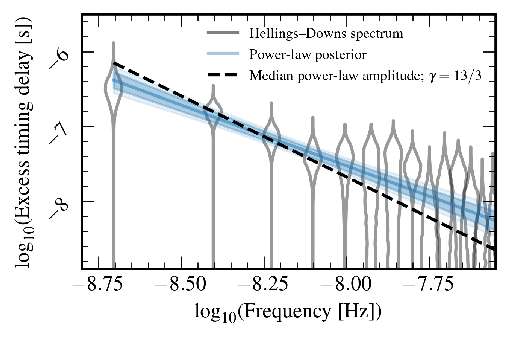
\includegraphics[width=.8\columnwidth]{thesisplots/ng15/nano15_hd_freespec_fig1}
	\caption{Results of a free-spectral analysis and fit to power-law \ac{GWB} signals of \ac{NANOGrav}’s 15-year data set. The gray violins represent \ac{GW} amplitudes' posteriors at different frequencies $f_k = k / T$. The dashed line indicates the best-fit \ac{GWB} power-law model with a fixed spectral index $\gamma = 13/3$. The blue bands represent the $1\sigma$ and $2\sigma$ posterior intervals for the power-law model with a variable spectral index. This figure was taken from ref.~\cite{NANOGrav:2023gor}.
		\label{fig:spectrum_correlations_plot}}
\end{figure}

Fig.~\ref{fig:spectrum_correlations_plot2} showcases the Bayesian reconstruction of the overlap reduction function for the common red noise. This function was modeled as a cubic spline, while a power-law with a variable spectral index $\gamma$ was used for the \ac{GWB}. The posterior \graffito{Bayesian reconstruction of the \ac{HD} curve} distributions of the overlap reduction function were computed at pre-selected positions, including the point of minimal \ac{HD} correlation at 49 degrees, the zero-crossings of the \ac{HD} curve, and the minimal and maximal angular separations. For reference, the \ac{HD} curve is shown as a dotted line.

\begin{figure}[t]
	\centering
	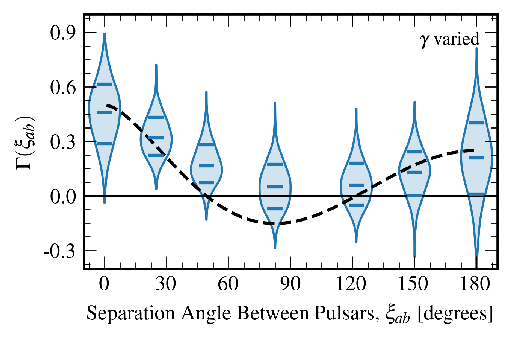
\includegraphics[width=.8\columnwidth]{thesisplots/ng15/nano15_splineorf_vg_violinplot_fig1}
	\caption{
		Bayesian reconstruction of the overlap reduction function for the common red noise signal in \ac{NANOGrav}’s 15-year data set. The blue violins display the posterior distributions of the overlap reduction function at selected separation angles, with the dashed line representing the expected \ac{HD} curve for a stochastic gravitational wave background. This figure was taken from ref.~\cite{NANOGrav:2023gor}.
		\label{fig:spectrum_correlations_plot2}}
\end{figure}

The robustness of these results was confirmed through various methods, including a separate frequentist analysis, a dropout analysis (leaving out some pulsars), and analyzing data from individual radio telescopes. While there is some dependence on the choice between the \acs{DMX} and \acs{DMGP} model for hyper-parameter inference, this does not affect the \graffito{Robustness of \ac{NANOGrav}'s findings} evidence for the \ac{HD} correlation~\cite{NANOGrav:2023gor}. The evidence for the \ac{GWB} is expected to increase further with time. The anticipated $5\sigma$ detection limit might already be achieved within the upcoming third \acs{IPTA} data release, which will combine datasets from \acs{NANOGrav}, \acs{EPTA}, \acs{InPTA}, and \acs{PPTA}, encompassing observations of 80 pulsars over a 24-year data span.

Following the \ac{PTA} announcements of 2023, a large number of articles studied a hypothetical cosmological origin of the novel signal. Possible origins of the \ac{PTA} signal include the \ac{GWB} emission through \acp{FOPT}~\cite{Nakai:2020oit, Ratzinger:2020koh, NANOGrav:2021flc, Bringmann:2023opz, Madge:2023cak} or merging primordial black holes~\cite{Depta:2023qst, Gouttenoire:2023nzr}, which we will investigate in depth in the following chapters of this thesis. Other\graffito{Cosmology or astrophysics?} hypothesized cosmological sources for the nano-Hertz signal include cosmic strings~\cite{Ellis:2023tsl, Buchmuller:2023aus, Blasi:2020mfx, Ellis:2020ena, Buchmuller:2020lbh}, domain walls~\cite{Gouttenoire:2023ftk}, tensor modes produced in inflation~\cite{Vagnozzi:2023lwo,Vagnozzi:2020gtf,Ashoorioon:2022raz}, scalar-induced \acp{GW}~\cite{Dandoy:2023jot}, the production of primordial black holes~\cite{DeLuca:2020agl, Kohri:2020qqd, Vaskonen:2020lbd,Unal:2020mts,Ashoorioon:2022raz} and long-lived turbulence after a strong first-order \ac{QCD} \ac{PT}~\cite{RoperPol:2022iel}. The arguably strongest contender of these explanations, each of which includes an extension of the \ac{SM} in one or the other way, is a stochastic background emitted by a population of \acp{SMBHB}, being the subject of the following section.

\section{Supermassive black hole binaries} \label{sec:SMBHBs}

In any part of the spectrum of stochastic \acp{GWB} within the nHz to kHz range, one expects astrophysical foregrounds with amplitudes between $h^2 \Omega_\gw \simeq 10^{-12} - 10^{-9}$, limiting the \graffito{Astrophysical \ac{GW} foregrounds} sensitivity to primordial backgrounds (cf.~fig.~4 of ref.~\cite{Ghoshal:2023pcx} and references therein). In this section we will discuss the astrophysical \ac{GWB} in the nHz range stemming from mergers of \acp{SMBHB}, i.e.~black holes with $M = 10^8 - 10^{10} \, M_\odot$, relevant for \ac{PTA} searches of primordial backgrounds.

There is general agreement that supermassive black holes reside at the centers of most large galaxies, observable primarily through their interactions with surrounding matter, for instance as quasars~\cite{Kormendy:1995er, Magorrian:1997hw}. Only in 2019, it was possible to for the first time \graffito{Supermassive black holes} directly observe the shadow of the supermassive black hole Sagittarius A* residing at the center of our own galaxy~\cite{EventHorizonTelescope:2019dse}, after the existence of a black hole at the center of our galaxy with $M = 4 \cdot 10^9 \, M_\odot$ was predicted already in the late 1990s by the 2020 Nobel laureates Andrea Ghez and Reinhard Genzel~\cite{Ghez:1998ph, Eckart:1996zz}. As the growth of cosmic structure occurs hierarchically, through mergers of smaller galaxies into larger ones, a series of black hole mergers is expected in the recent cosmic history, giving rise to a stochastic \ac{GWB}.

The \ac{GWB} signal from \acp{SMBHB} is still a subject of active research and several key processes have not been fully understood, yet: For instance, it is still unclear how a large population of supermassive black holes can form given the maximal speed of accretion set by the Eddington formula~\cite{Volonteri:2021sfo}, a challenge known as the timing problem. \graffito{Open problems concerning \acsp{SMBHB}} Moreover, the merger process itself is complicated by the so-called final parsec problem~\cite{Binney:1987, Milosavljevic:2002ht, Dosopoulou:2016hbg}. While the existence of many \acp{SMBHB} with separations ranging from hundreds to thousands of parsecs have been observed in multi-messenger astronomy~\cite{DeRosa:2019myq}, the closest observed pair of supermassive black holes was still separated by roughly $7 \, \text{pc}$~\cite{Rodriguez:2006th}. For binaries to emit \acp{GW} in the nHz band, however, separations at the milliparsec-scale are required, which current optical telescopes are far from being able to resolve.

\subsection{Binary evolution and the final parsec problem} \label{sec:finalpc}

The main process assumed to dominate the hardening (i.e., the dissipation of binding energy) of a binary system with kiloparsec to parsec separations is dynamical friction. It is sourced by viscous drag forces of \acp{SMBHB} from many weak and long-range gravitational scatterings with smaller bodies. \graffito{Dynamical friction $\mathrm{(kpc}-\mathrm{pc)}$} This inspiral down to a parsec between the black holes takes roughly $\mathcal{O}(\text{Gyr})$ times~\cite{Binney:1987, Dosopoulou:2016hbg}. At lower distances, dynamical friction ceases to be efficient because of the increased radial velocity of the binary \acp{SMBHB}.

Below parsec separations, a process known as stellar loss-cone scattering becomes relevant instead. In this process, individual stars close to the galactic core are scattered out of the central region due \graffito{Stellar loss-cone scattering $\mathrm{(}\lesssim 1 \, \mathrm{pc)}$} to a gravitational slingshot mechanism. The hardening of the binary hence continues until this reservoir of stars within the so-called loss-cone is depleted. The original definition of the final parsec problem was the stalling of the binary evolution at this stage. Today, there are several pieces of evidence supporting the claim that there is an ongoing supply of stars in the post-merger galaxy~\cite{Vasiliev:2013az, Vasiliev:2013nha, Vasiliev:2015}.

At even lower separations of a hundredth to a thousandth of a parsec, viscous dissipation of binding energy \graffito{Viscous dissipation $\mathrm{(}\lesssim 10 \, \mathrm{mpc)}$} to the gaseous circumbinary disk could become important. It is, however, not yet clear whether this process actually hardens the binary~\cite{Ivanov:1998qk, Haiman:2009te} or rather widens it~\cite{Kocsis:2010xa}, giving rise to a new final parsec problem. Another interesting mechanism, which however requires new physics, acting at the same distance scales is dynamical friction of a self-interacting \ac{DM} fluid surrounding the \ac{SMBHB}~\cite{Alonso-Alvarez:2024gdz}. 

If a binary can pass this barrier and hardens down to below-milliparsec separations, the binary evolution decouples from astrophysical interactions and instead becomes driven by \ac{GW} emission alone until the black holes coalesce at microparsec separations. \graffito{GW emission until coalescence $\mathrm{(mpc}-\mathrm{\mu pc)}$} It has been proposed that another mechanism might contribute to the hardening of binaries, through so-called triplet interactions with a close-by third supermassive black hole~\cite{Amaro-Seoane:2009ucl}. It appears reasonable that in the process of hierarchical structure formation, a third galaxy might come close to the binary whose orbit then becomes more eccentric, which accelerates its coalescence due to an increased \ac{GW} emission. In fact, this will be the mechanism which will ensure a solution of the final parsec problem for the merging \acp{PBH} considered in chapter~\ref{chp:pbh}. To date the final parsec problem has not been solved on theoretical grounds. Given the recent advances of \acp{PTA} it is however conceivable that the underlying mechanism can  be inferred through the emitted \ac{GW} spectrum, which we will discuss in the the following section.

\subsection{GWBs from inspiraling binaries}

Assuming that the final parsec problem can be resolved, the \ac{GWB} from a population of \acp{SMBHB} could explain the measured nHz background~\cite{NANOGrav:2023hfp}. We will now briefly review how a power-law spectrum can be derived from simple scaling \graffito{A simple power-law} relationships and where possible deviations from it can stem from. The introduced formalism will be used in chapter \ref{chp:pbh}, in which we will test the assumption that the novel signal stems from inspiraling \acp{SMBHB} of primordial origin.

Any isotropic background from a large enough compact binary population can be expressed as~\cite{Maggiore:2018sht}
\begin{align}
	h^2 \Omega_\gw(f) &= \frac{h^2}{\rho_\crit^0} \td{\rho_\gw}{\log f} = \frac{h^2}{\rho_\crit^0} \int_0^\infty \diff z \, \td{n}{z} \frac{1}{1 + z} \left.\td{E_\gw^\text{r}}{\log f_\text{r}} \right|_{f_\text{r} = f(1 + z)} \, , \label{eq:binaryGW}
\end{align}
where $\diff n / \diff z$ is the number density distribution of binaries over redshift $z$, $\diff E_\gw^\text{r} / \diff \log f_\text{r}$ is the \graffito{Summing over sources and integrating over the expansion history} source-frame \ac{GW} energy spectrum per logarithmic frequency interval, $f_\text{r} = f(1+z)$ is the \ac{GW} frequency in the source frame, and the factor $1/(1+z)$ accounts for the redshift of the energy $E_\gw = E_\gw^\text{r}/(1 + z) $ to today. The interpretation of the above equation is straightforward: to find the amplitude of the  \ac{GW} spectrum at a frequency $f$, we sum over all contributions from binaries emitting frequencies $f_\text{r}$ corresponding to a frequency $f$ today and then integrate over the cosmic expansion history.

To get a feeling for the quantities involved in eq.~\eqref{eq:binaryGW} let us first compute the expected frequency dependence of the spectrum $\diff E_\gw^\text{r} / \diff f_\text{r}$ for a single binary. In the weak-field limit of small velocities and at large radial separations $r$ from the binary, the \graffito{The quadrupole formula} \ac{GW} equation of motion~\eqref{eq:GW} can be solved by the famous quadrupole formula~\cite{Maggiore:2007ulw}
\begin{align}
	&h_{ij}^\TT= \frac{\Lambda_{ij, kl}}{4 \pi \Mp^2 r}  \ddot{Q}_{kl}\ba{t-\frac{r}{c}} \quad \text{with}  \quad \Lambda_{ij,kl}(\hat{\bm{n}}) = P_{ik} P_{jl} - \frac{1}{2}P_{ij} P_{kl} \nonumber \\ &\text{and}
	\qquad Q_{ij} = \int \diff^3 x \, \rho(t, \bm{x}) \ba{x_i x_j - \frac{1}{3} \delta_{ij} r^2} ,
\end{align}
where $\Lambda_{ij,kl}(\hat{\bm{n}})$ is simply known as the $\Lambda$-tensor. It can be expressed through the tensor $P_{ij}(\hat{\bm{n}}) \equiv \delta_{ij} - n_i n_j$ and it is commonly used to project out the \ac{TT}-part of tensors. A derivation of the above equation can for instance be found in chapter 3 of ref.~\cite{Maggiore:2007ulw}. Assuming that the binary consists of two compact objects of mass $M$ on a stable circular orbit with \graffito{$\omega_\mathrm{gw}= 2 \omega$} radius $R$ in the $x$-$y$ plane and orbital frequency $\omega$, one obtains
\begin{align}
	h_{ij}^\TT = - \frac{M R^2 \omega^2}{\pi \Mp^2 r} \begin{pmatrix}
		\cos 2 \omega t & \sin 2 \omega t &0\\
		\sin \omega t &- \cos 2 \omega t &0\\ 
		0 &0 &0
	\end{pmatrix} . \label{eq:GWbinary}
\end{align}
Using the stress-energy tensor of a \ac{GW} from eq.~\eqref{eq:stressenergy} one can obtain an expression for the energy loss of the binary through \ac{GW} emission per unit solid angle. \graffito{The luminosity in \acp{GW}} Integrating over a large enough sphere around the binary, one obtains the gravitational luminosity of the source
\begin{align}
	P_\text{gw} = \td{E_\gw^\text{r}}{t_\text{r}} = \frac{\langle \dddot{Q}_{ij} \dddot{Q}^{ij} \rangle }{40 \pi \Mp^2}  \propto G M^2 R^2 \omega^2 \propto G^{7/3} M^{10/3} \omega^{10/3} \, ,
\end{align}
where in the last step we used Kepler's law $\omega^2 = \frac{GM}{4 R^3}$ to eliminate the $R$-dependence. Obviously, this radiative energy loss will reduce the binding energy $E_\text{b} \propto G M^2 / R$ of the binary, thus hardening the binary. Working in the limit that this radiative energy loss takes place on much longer timescales than the orbital motion, we can still treat the orbits as quasi-circular and equate $\dot{E}_\text{b} = P_\gw$ in the cosmic rest-frame of the binary. Plugging in Kepler's law another time to eliminate $R$ in favor of $\omega$ and using the previously derived expression for $P_\gw$, one immediately arrives at $\dot{\omega} \propto G^{13/3} M^{17/3} \omega^{11/3}$.

Realizing that the \ac{GW} frequency is proportional to the orbital frequency, $2 \pi f_\text{r} = 2 \omega$ (see eq.~\ref{eq:GWbinary}), we can hence perform the simple approximation for the spectrum emitted by a compact binary 
\begin{align}
	\td{E_\gw^\text{r}}{\log f_\text{r}} = f_\text{r} \td{E_\gw^\text{r}}{t_\text{r}} \td{t_\text{r}}{f_\text{r}} \propto f_\text{r} \times f_\text{r}^{10/3} \times f_\text{r}^{-11/3} = f_\text{r}^{2/3} . \label{eq:13/3}
\end{align}
Since this expression carries the full frequency dependence of eq.~\eqref{eq:binaryGW}, we find that $h^2 \Omega_\gw(f) \propto f^{2/3}$ or equivalently $h_\text{c} \propto f^{-2/3}$ and $\Phi(f) \propto f^{-13/3}$ (cf.~eq.~\eqref{eq:Phif}). The exponents of $h_\text{c}(f)$ and $\Phi(f)$ are usually referred to as $\alpha = -2/3$ and $\gamma = 2-2\alpha = 13/3$, respectively.  In fact, the proportionalities derived above also hold \graffito{$\gamma = 13/3$} for a general circular orbit of compact binaries with different masses, which was first appreciated by Phinney in his influential article from 2001~\cite{Phinney:2001di}.

Of course, the above scaling can only hold in a finite frequency window as otherwise the energy carried in the \ac{GWB} spectrum were unbounded: At an initial state of the inspiral, the hardening of the binary will be mostly driven by environmental effects, such that the spectrum will bend down towards lower spectral amplitudes at low frequencies. The high-frequency part of the spectrum is emitted by the inspiral of binaries just before coalescence. The \graffito{Deviations from $\gamma = 13/3$} highest possible \ac{GW} frequency emitted through the inspiral of a binary hence corresponds to the so-called innermost stable circular orbit and is given by
$f_\text{ISCO}^\text{r} = 4.7 \cdot 10^{-7} \, \text{Hz} \, \ba{10^{10} \, M_\odot / M }$, cf.~eq.~(16.78) in ref.~\cite{Maggiore:2018sht}. For a monochromatic mass spectrum the of \acp{SMBHB}, this would correspond to a sharp cutoff of the spectrum lying above the \acp{PTA} frequency band. In reality, however, the number density distribution $\diff n / \diff z$ in eq.~\eqref{eq:binaryGW} will depend on the distribution of \ac{SMBHB} masses, softening the decrease of the spectrum at high frequencies. Special attention needs to be paid due to the finiteness of the distribution of black holes with extremely high masses: there needs to be at least one source in order to emit a \ac{GW} signal. We will investigate this issue in more detail in chapter~\ref{chp:pbh}, see e.g.~fig.~\ref{fig:res_explanation}.

\begin{figure}
	\centering
	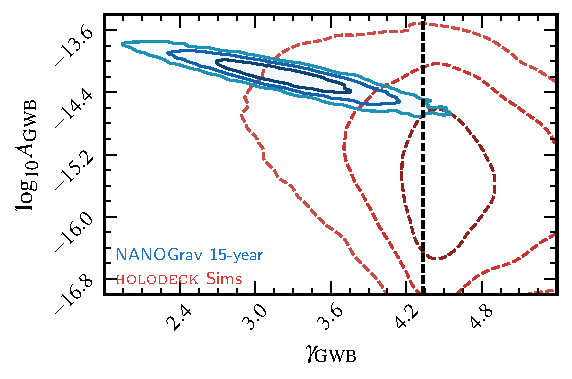
\includegraphics[width=0.8\linewidth]{thesisplots/ng15/nano15_astrogw_compare}
	\caption{Marginalized posterior distributions of the amplitude $A$ and spectral index $\gamma$ for power-law fit of the \ac{HD}-correlated red noise in the \ac{NANOGrav} 15yr data set compared to predictions obtained using the \texttt{Holodeck} code for an \ac{SMBHB}-induced background. The vertical line at $\gamma = 13/3$ refers to a population of \acp{SMBHB} whose inspiral is driven only by \ac{GW} emission. This figure was taken from ref.~\cite{NANOGrav:2023hvm}.}
	\label{fig:nano15astrogwcompare}
\end{figure}


The \ac{NANOGrav} collaboration uses the code \texttt{Holodeck}~\cite{NANOGrav:2023gor} to generate \ac{GWB} spectra from \acp{SMBHB} based on realistic astrophysical distributions, starting from galaxy merger rates and black hole-host galaxy mass relationships. Recently, a phenomenological model for those \ac{GWB} spectra has been put forward which allows the inference of black hole properties~\cite{NANOGrav:2023hfp}. In doing so, it \graffito{\ac{NANOGrav} vs. \acp{SMBHB}} was found that several astrophysical quantities like the binary hardening timescale need to be beyond the borders of their previously expected ranges in order to explain the observed \ac{GWB} spectrum at nHz frequencies~\cite{NANOGrav:2023hfp}. In fig.~\ref{fig:nano15astrogwcompare}, a comparison of the expected amplitude and spectral tilt of the spectrum based on \texttt{Holodeck} simulations and the regions of parameter space preferred by the \ac{NANOGrav} 15yr data set can be found. Even though the tension between the contours of prediction and expectation still depends on the used priors of the astrophysical simulations, the figure already indicates that there is room (if not the necessity) for an additional \ac{GW} source which also contributes to the observed nHz signal. This serves as a source of motivation when searching for alternative explanations of the signal in the following chapters \ref{chp:ptabbn} and \ref{chp:pbh}.

